\documentclass{standalone}
\usepackage{pgfplots}

\begin{document}



\tikzset{every picture/.style={line width=0.75pt}} %set default line width to 0.75pt        

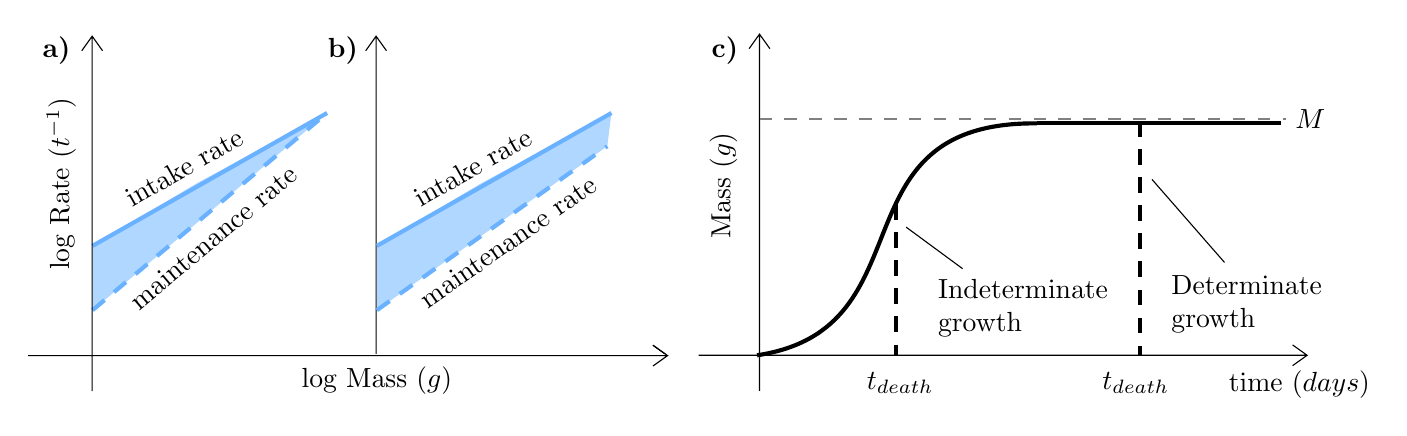
\begin{tikzpicture}[x=0.75pt,y=0.75pt,yscale=-1,xscale=1]
%uncomment if require: \path (0,300); %set diagram left start at 0, and has height of 300

%Shape: Axis 2D [id:dp6270801068910796] 
\draw  (153,207.9) -- (309,207.9)(168.6,54) -- (168.6,225) (302,202.9) -- (309,207.9) -- (302,212.9) (163.6,61) -- (168.6,54) -- (173.6,61)  ;
%Shape: Polygon [id:ds4708755381223775] 
\draw  [draw opacity=0][fill={rgb, 255:red, 175; green, 215; blue, 255 }  ,fill opacity=1 ] (219,125) -- (282,91) -- (280,107) -- (169,186) -- (169,155) -- cycle ;
%Shape: Polygon [id:ds9632747098248329] 
\draw  [draw opacity=0][fill={rgb, 255:red, 175; green, 215; blue, 255 }  ,fill opacity=1 ] (82,125) -- (145,91) -- (81,145) -- (32,186) -- (32,155) -- cycle ;
%Shape: Axis 2D [id:dp1042623091180761] 
\draw  (324,207.73) -- (617.17,207.73)(353.32,53) -- (353.32,224.92) (610.17,202.73) -- (617.17,207.73) -- (610.17,212.73) (348.32,60) -- (353.32,53) -- (358.32,60)  ;
%Curve Lines [id:da33454180544837087] 
\draw [color={rgb, 255:red, 0; green, 0; blue, 0 }  ,draw opacity=1 ][line width=1.5]    (352.15,207.73) .. controls (436.61,195) and (387.1,95) .. (487.09,96) ;


%Straight Lines [id:da738837712532068] 
\draw [color={rgb, 255:red, 0; green, 0; blue, 0 }  ,draw opacity=1 ][line width=1.5]    (487.09,96) -- (604.81,96) ;


%Straight Lines [id:da8136832978580617] 
\draw [color={rgb, 255:red, 0; green, 0; blue, 0 }  ,draw opacity=1 ][line width=1.5]  [dash pattern={on 5.63pt off 4.5pt}]  (536.6,95) -- (536.6,208) ;


%Straight Lines [id:da8829084110612089] 
\draw [color={rgb, 255:red, 0; green, 0; blue, 0 }  ,draw opacity=1 ][line width=1.5]  [dash pattern={on 5.63pt off 4.5pt}]  (419.13,135) -- (419.13,208) ;


%Straight Lines [id:da21752989570784442] 
\draw    (423.99,146) -- (451.17,166) ;


%Straight Lines [id:da8434950124235723] 
\draw    (577.37,163) -- (542.42,123) ;


%Straight Lines [id:da19163379879655684] 
\draw [color={rgb, 255:red, 128; green, 128; blue, 128 }  ,draw opacity=1 ][line width=0.75]  [dash pattern={on 4.5pt off 4.5pt}]  (353.36,94) -- (607.09,94) ;


%Straight Lines [id:da025683092509892314] 
\draw [color={rgb, 255:red, 106; green, 178; blue, 255 }  ,draw opacity=1 ][line width=1.5]    (32,155) -- (145,91) ;


%Straight Lines [id:da8885553496340661] 
\draw [color={rgb, 255:red, 106; green, 178; blue, 255 }  ,draw opacity=1 ][line width=1.5]  [dash pattern={on 5.63pt off 4.5pt}]  (32,186) -- (145,91) ;


%Straight Lines [id:da9765394894099406] 
\draw [color={rgb, 255:red, 106; green, 178; blue, 255 }  ,draw opacity=1 ][line width=1.5]    (169,155) -- (282,91) ;


%Straight Lines [id:da806330594216591] 
\draw [color={rgb, 255:red, 106; green, 178; blue, 255 }  ,draw opacity=1 ][line width=1.5]  [dash pattern={on 5.63pt off 4.5pt}]  (169,186) -- (280,107) ;


%Shape: Rectangle [id:dp2541433612704507] 
\draw  [draw opacity=0][fill={rgb, 255:red, 255; green, 255; blue, 255 }  ,fill opacity=1 ] (135,207) -- (309,207) -- (309,232) -- (135,232) -- cycle ;
%Shape: Axis 2D [id:dp7084513866375908] 
\draw  (1,207.9) -- (309,207.9)(31.8,54) -- (31.8,225) (302,202.9) -- (309,207.9) -- (302,212.9) (26.8,61) -- (31.8,54) -- (36.8,61)  ;

% Text Node
\draw (534.65,221) node  [align=left] {$t_{death}$};
% Text Node
\draw (421.08,221) node  [align=left] {$t_{death}$};
% Text Node
\draw (480.29,185) node  [align=left] {Indeterminate\\growth};
% Text Node
\draw (588.05,183) node  [align=left] {Determinate\\growth};
% Text Node
\draw (613.47,222) node  [align=left] {time ($days$)};
% Text Node
\draw (618.65,94) node  [align=left] {$M$};
% Text Node
\draw (76,117) node [rotate=-330.52] [align=left] {intake rate};
% Text Node
\draw (215,117) node [rotate=-330.52] [align=left] {intake rate};
% Text Node
\draw (90,151) node [rotate=-320] [align=left] {maintenance rate};
% Text Node
\draw (232,153) node [rotate=-325] [align=left] {maintenance rate};
% Text Node
\draw (169,220) node  [align=left] {log Mass ($g$)};
% Text Node
\draw (17,125) node [rotate=-270] [align=left] {log Rate ($t^{-1}$)};
% Text Node
\draw (336,126) node [rotate=-270] [align=left] {Mass ($g$)};
% Text Node
\draw (14.65,61) node  [align=left] {\textbf{a)}};
% Text Node
\draw (152.65,61) node  [align=left] {\textbf{b)}};
% Text Node
\draw (336.65,61) node  [align=left] {\textbf{c)}};


\end{tikzpicture}

\end{document}